\documentclass[times, 10pt, twocolumn]{article}
\usepackage{amsmath,amsfonts,amsthm,amssymb}
\usepackage{fancyhdr}
\usepackage{chngpage}
\usepackage{color}
\usepackage{graphicx}
\usepackage{boxedminipage}
\usepackage{enumerate}
\usepackage{latex8}
\usepackage{times}
\usepackage[utf8]{inputenc}

\rfoot{Page \thepage \hspace{1pt} of \pageref{LastPage}} %Talvez tire a numeracao tendo em conta que eles nao a poe no template

\title{DADSTORM\\A simple, fault-tolerant and real-time stream processing system}
\author{DAD 2016-2017\\ Group 12:
\\ Daniel Fermoselle nº 78207
\\ João Marçal nº 78471
\\ Tiago Rodrigues nº 78692
}
\begin{document}
\maketitle
\date

\begin{abstract}
DADSTORM is a simple but reliable stream processing system. It's mainly used by Instituto Superior Tecnico Students.
\\The main features are: the 3 possible semantics of tuple processing it can have, fault-tolerance to f faults per operator with a synchronous model of detection, 3 modes of tuple routing and last but the not the least 
5 types of operators.
This system is composed by a Puppet Master, Process Creation Service, Operators with their Replicas, Tuples and ThreadPools.
\end{abstract}

%------------------------------------
\section{Introduction}
Nowadays with the rising interest on big data streaming information is getting more and more important and we want to process that data as fast as possible even though existing the possibility of having faults. 
In order to get that information in a reliable way we developed DADSTORM. This system is reliable through the passive replication we use, allowing us to get tolerance to f faults using just f+1 replicas. 
\\Our system process tuples based on the type of operator which can be UNIQ, COUNT, DUP, FILTER and CUSTOM. With these operators we can get the data processed in a way that let us get the information we want.

%------------------------------------
\section{Programming Model}
In this section, we provide a high-level overview of the programming model, highlighting the key concepts. 
\\In DADSTORM data is represented as string Tuples, i.e, a collection of strings.
\\To begin with we have a puppet master who will start all the operators on all the machines with the help of the process creation service this last will already be located in all the machines that will run operator replicas.
\\The puppet master has an intuitive interface inside which we have a box where we can introduce a path to a configuration file (see figure 1) to start all the operator's replicas as well has their inputs, routing, operator spec and address.
\begin{figure}
  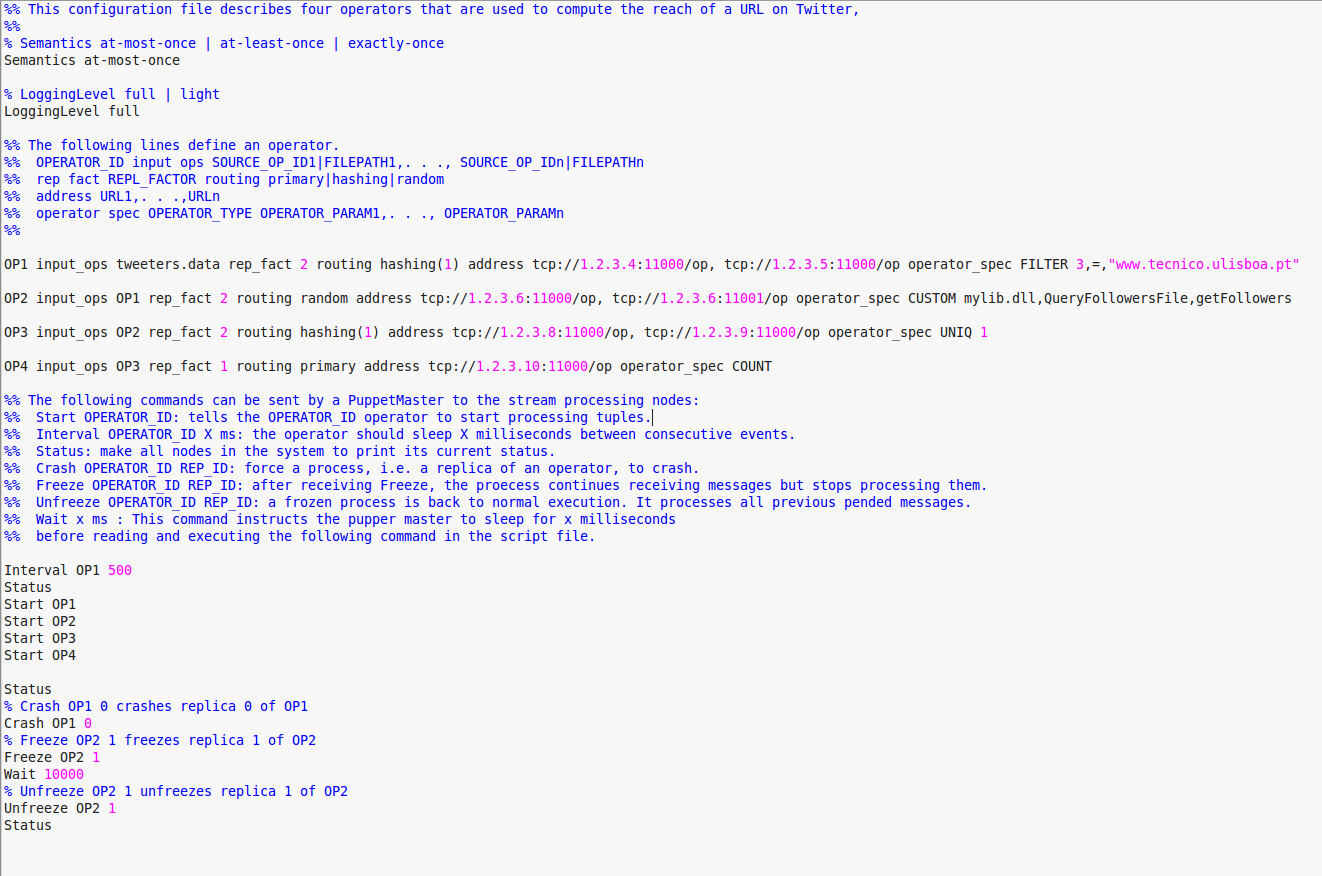
\includegraphics[width=\linewidth]{configFileExample.PNG}
  \caption{An example of a config file.}
\end{figure}
\\The tuples are stored inside a file that will be accessed by the first operator of the stream. The operators are composed by replicas which can be located inside different machines.
\\All the replicas might fail but we assure f fault tolerance to silent failures for each operator. We assume that none of the first operator replicas can fail and that there is at least one replica alive per operator, in order to guarantee that to be possible we have to have at least f+1 replicas for each operator, being f the number of fautls of each operator.
\\A quick overall. So first of all we start the puppet master which will through the configuration file introduced and with the help of the process creation service create all the operator's replicas. Then the replicas of the first operator will read the .dat file which has the begining tuples to be processed. After this initialization all the replicas will receive tuples and process them, sending the result to the next operators, unless it is a replica of the last operator this one doesn't send anything, it just processes tuples.
\\To finish this section the user of our system doesn't have to worry about how the system is distributing the operations, the user just has to create the configuration file and let the puppet master read it, then just execute and all the data will be processed, getting in the end the desired information.



%------------------------------------
\section{DADSTORM Abstractions}
In this section we will talk a little bit about the abstractions we created for this system, begining with the tuple and all its variations, having an overview about the operator, the replicas. To finish the section we will talk about the parser, the RepInfo and the ConfigInfo.



%------------------------------------
\subsection{Tuple}
Tuple, this is one of the most important abstractions of our system if not the most one. The Tuple is a possible infinite collection of strings, it also has a unique id to be used when the tuple processing semantics requires so. The tuples are processed and when this happens it is created another tuple having as content the result of processing the previous tuple. 
\\To help mostly the processing semantics we created also 3 more variations of the tuple, which are: AckTuple, TimerTuple and Tuple2TupleProcessed. 
\\The AckTuple is no more than a tuple associated with the url of the replica who sent the tuple this url can be used in the future. 
\\The TimerTuple is a tuple associated with a timer of the limit the tuple has to be acked otherwise it'll be resent. 
\\Last but not the least there is the Tuple2TupleProcessed this abstraction contains 2 tuples, the first tuple when processed by some replica generates the second tuple, this association can be useful first to compare if the tuple was already processed and then to return the result of processing the first tuple if necessary.



%------------------------------------
\subsection{Operators and Replicas}
In this section we will talk mostly about replicas because they are simply what an operator is.
\\A replica basically is an object that reads tuples from possibly infinite inputs, processes and finally sends them to the next replicas in the chain.
\\Each replica has a thread pool which will have 2 threads one for reading tuples and processing them and another thread to send the processed tuples to the next replicas. Each thread has a circular buffer in which the tuples will be waiting to be read and processed or sent. The replicas also have a RepInfo that will be defined below. A replica also has a status, 
\\TODO FINISH



%------------------------------------
\subsection{Parser}
The parser is an abstraction used by the puppet master in order to process the configuration file, this parser receives the path to the configuration file and gives to the puppet master an array of ConfigInfo with all the information of the operators and its replicas as well as the list of commands that the puppet master will have to execute.
\\TODO VERIFICAR



%------------------------------------
\subsection{RepInfo}
RepInfo is an abstraction that basically gives all the information that a replica of an operator has to know. It has the notion of replica routing, its parameters as well as the urls of the replicas to which will be sent tuples, the url of the replica, the operator spec i.e what operation the replica will perform, the id of the replica, the sibling replicas i.e the replicas from the same operator. 
\\In short the RepInfo has all the information that a replica needs to know.
\\TODO SERA NECESSARIO ADICIONAR MAIS COISAS?




%------------------------------------
\subsection{ConfigInfo}
This abstraction is almost the same as the RepInfo but for the puppet master. It's through the ConfigInfo that the puppet master can know how to start the replicas with which properties that in the correct time will be sent to the replicas inside the RepInfo



%------------------------------------
\subsection{Failure Recovery}
To guarantee failure recovery some of the previous abstractions will be used, but how this is done will be explained in section 4. Some recovery techniques use the Timer Tuples as well as the RepInfo as we will see below.



%------------------------------------
\section{Architecture and Implementation}
In this section we will describe in more detail what each component of the architecture of our solution does and how it was implemented.




%------------------------------------
\subsection{Tuple}
As said in section 3.1 the tuple is the base of our whole system. The tuple contains a collection of strings and an unique id, this id is composed by the operator name concatenated with the replica index plus an unique id inside that replica. This first basic tuple is sent between replicas and gets changed every time it's processed. The AckTuple is the first sub-type of tuples and each operator saves an array list with this object until the tuple is acked, this sub-type plus the TimerAck which has the timer to receive ack before resend the tuple work together to guarantee that the tuple is at least received once. Now the last sub-type of tuple is Tuple2TupleProcessed this tuple saves the pair \textless Tuple, TupleProcessed\textgreater and it's used as a method to let the replica know if the tuple was already processed comparing the id's of the tuple receive and all the pairs Tuple2TupleProcessed saved in an array in each replica.



%------------------------------------
\subsection{Operators and Replicas}
The notion of operator is as said before a little bit abstracted as a collection of replicas, that being said in this subsection we will only talk about replicas. 
\\The key of the replicas is to mantain state as well as tracking all the tuples.
\\Replicas are implemented as object which have a few structures inside: one threadpool, one RepInfo, one status and a few array lists that will be explained in the end of this sub-section.
\\First of all the threadpool, this atribute mantains a reference to access the replica threadpool that has 2 threads: one to read and process and another to send tuples. Each of this threads has a circular buffer where the tuples are stored while waiting to be consumed. When the circular buffer gets full it will block the reception until there is a consume action. One of the threads will be constantly running a ConsumeRead method that consumes tuples from the circular buffer reads it and with the replica operator spec processes it, after that, the tuple is sent to the circular buffer of the thread which is always running a ConsumeProcessed method, this thread will take a tuple from its circular buffer and with the replica is going to send to the right next replica.
\\The RepInfo this structure has a lot of information for one replica(this replica), more specifically: \textbf{routing}, the type of routing for this replica, \textbf{routingParam}, the parameters of the tuple to which the routing will be applied in this replica, \textbf{nextRouting}, the type of routing for the possible next replicas, \textbf{nextRoutingParam},the parameters of the tuple to in which the routing will be applied in the possible next replicas, \textbf{operatorSpec}, the type of this replica operator, \textbf{operatorParam}, the parameters of the tuple on which this replica operatorSpec will be applied, \textbf{sendInfoUrls}, the urls of the next replicas, \textbf{port}, this replica port, \textbf{loggingLvl},the type of logging that the system is configured for, \textbf{input}, the input operators or file of this replica, this is mainly used to get the file.dat, \textbf{pmsUrl}, the url of the puppet master, \textbf{siblingsUrls},the urls of the other replicas of the same operator,  \textbf{myUrl}, the url of this replica,   \textbf{semantics}, the semantics the system in running,  \textbf{receiveInfoUrls}, the urls of the replicas which can send tuples to this replica, \textbf{operatorId} the id of this replica's operator. With all this information the system can know which replicas should have the copy of the state in case of failure (siblings), which replicas will receive the tuples processed (sendInfoUrls), the type of operator (operator spec).
\\The status of a replica indicates if it's working or not and there is also information about the replica being frozen.
\\ArrayLists ...





%------------------------------------
\subsection{Puppet Master}
The puppet master provides an interface between the system and the user
//TODO WHAT TO SAY




%------------------------------------
\subsection{Process Creation Service}
The process creation service was created just to allow the puppet master to contact him through the shared common class which allow the puppet master to create the replicas of the operators in the machines where the process creation service is running.



%------------------------------------
\subsection{Failure Recovery}
Our system as already said has f+1 replicas per operator in order to guarantee faul-tolerance to f silent failures. This is guaranteed in a synchronous model because each replica has two timers, one that every 12 seconds sends a ping to the replica siblings, i.e the replicas that are part of the same operator, and another that every 12 seconds sends a ping to the replica children, i.e the replicas that receive tuples from this one.
\\If the first ping doesn't get response from one sibling that sibling is removed from the list and all the tuples that were being saved in shared array of replicated tuples are reprocessed and sent to the right receiving operator's replica.
\\Now about the second timer, if a child doesn't ping back it's simply removed from the possible sendInfoUrl, i.e the possible urls of replicas that can receive tuples from this one, in order to forbid the sender to wrongly send tuples to a dead replica.





%------------------------------------
\section{Discussion}




%------------------------------------
\section{Production Experiences}





%------------------------------------
\section{Evaluation}






%------------------------------------
\section{Conclusion}



\end{document}
